% !TEX encoding = UTF-8 Unicode.

% Based on https://github.com/Miracle0565/BUCT-Beamer-Theme

\documentclass[
10pt,
aspectratio=43,
]{beamer}
\setbeamercovered{transparent=10}
\usetheme[
%  showheader,
%  red,
  purple,
%  gray,
%  graytitle,
  colorblocks,
%  noframetitlerule,
]{Verona}

\usepackage[T1]{fontenc}
\usepackage{tikz}
\usepackage[utf8]{inputenc}
\usepackage{lipsum}
%%%%%%%%%%%%%%%%%%%%%%%%%%%%%%%
% Mac上使用如下命令声明隶书字体, windows也有相关方式, 大家可自行修改
\providecommand{\lishu}{\CJKfamily{zhli}}
%%%%%%%%%%%%%%%%%%%%%%%%%%%%%%%
\usepackage{tikz}
\usetikzlibrary{fadings}
%
%\setbeamertemplate{sections/subsections in toc}[ball]
\usepackage{xeCJK}
\usepackage{listings}
\usepackage{caption}
\usepackage{subfigure}
\usefonttheme{professionalfonts}
\def\mathfamilydefault{\rmdefault}
\usepackage{amsmath}
\usepackage{multirow}
\usepackage{booktabs}
\usepackage{bm}
\setbeamertemplate{section in toc}{\hspace*{1em}\inserttocsectionnumber.~\inserttocsection\par}
\setbeamertemplate{subsection in toc}{\hspace*{2em}\inserttocsectionnumber.\inserttocsubsectionnumber.~\inserttocsubsection\par}
\setbeamerfont{subsection in toc}{size=\small}
\AtBeginSection[]{%
	\begin{frame}%
		\frametitle{Outline}%
		\textbf{\tableofcontents[currentsection]} %
	\end{frame}%
}

\AtBeginSubsection[]{%
	\begin{frame}%
		\frametitle{Outline}%
		\textbf{\tableofcontents[currentsection, currentsubsection]} %
	\end{frame}%
}

\title{高等数学C: 回顾极限}
%\subtitle{A Simple while elegant template}
\author[P.Yu]{余沛}
\mail{peiy\_gzgs@qq.com}
\institute[Guangzhou College of Technology and Business]{Guangzhou College of Technology and Business \\
  广州工商学院}
\date{\today}
\titlegraphic[width=4cm]{logo.png}{}




%%%%%%%%%%%%%%%%%%%%%%%%%%%%%%%%
% ----------- 标题页 ------------
%%%%%%%%%%%%%%%%%%%%%%%%%%%%%%%%



\begin{document}

\maketitle

%%% define code
\defverbatim[colored]\lstI{
    \begin{lstlisting}[language=C++,basicstyle=\ttfamily,keywordstyle=\color{red}]
	int main() {
	// Define variables at the beginning
	// of the block, as in C:
	CStash intStash, stringStash;
	int i;
	char* cp;
	ifstream in;
	string line;
	[...]
	\end{lstlisting}
}
%%%%%%%%%%%%%%%%%%%%%%%%%%%%%%%%
% ----------- FRAME ------------
%%%%%%%%%%%%%%%%%%%%%%%%%%%%%%%%
\section{直与曲的梦乡}
\begin{frame}{开普勒:测量酒桶}
    \begin{columns}
        \column{0.5\textwidth}
        开普勒 (Johannes Kepler, 1571-1630) 在《求酒桶体积之新法》 (Novastereometria doliorum vinariorum, 1615, Ostwalds Klassiker) 考察酒桶体积以确定酒桶最佳形状时, 将木桶体积看成由一层层薄片组成. 当薄片足够薄, 那么酒桶的体积就应该是薄片体积的和.\\
        \pause
        \vspace{0.5cm}
        但这也出现了一个问题问题, 酒桶的表面积并不能简单地看作是薄片的表面部分的叠加($\pi\neq4$!). \pause 更合理的观察方法是酒桶面的侧面叠加.\\
        \pause
        \vspace{0.5cm}
        {\small \color{blue}
            可以看到, 由于用三角形的两边和讨论第三边长度是不合适的, 因此需要计算夹角值, 也就导出了所谓的微商的定义.\\
            \pause
            \vspace{0.1cm}
            (微商几何意义: 斜率)
        }
        \column{0.5\textwidth}
        \begin{figure}
            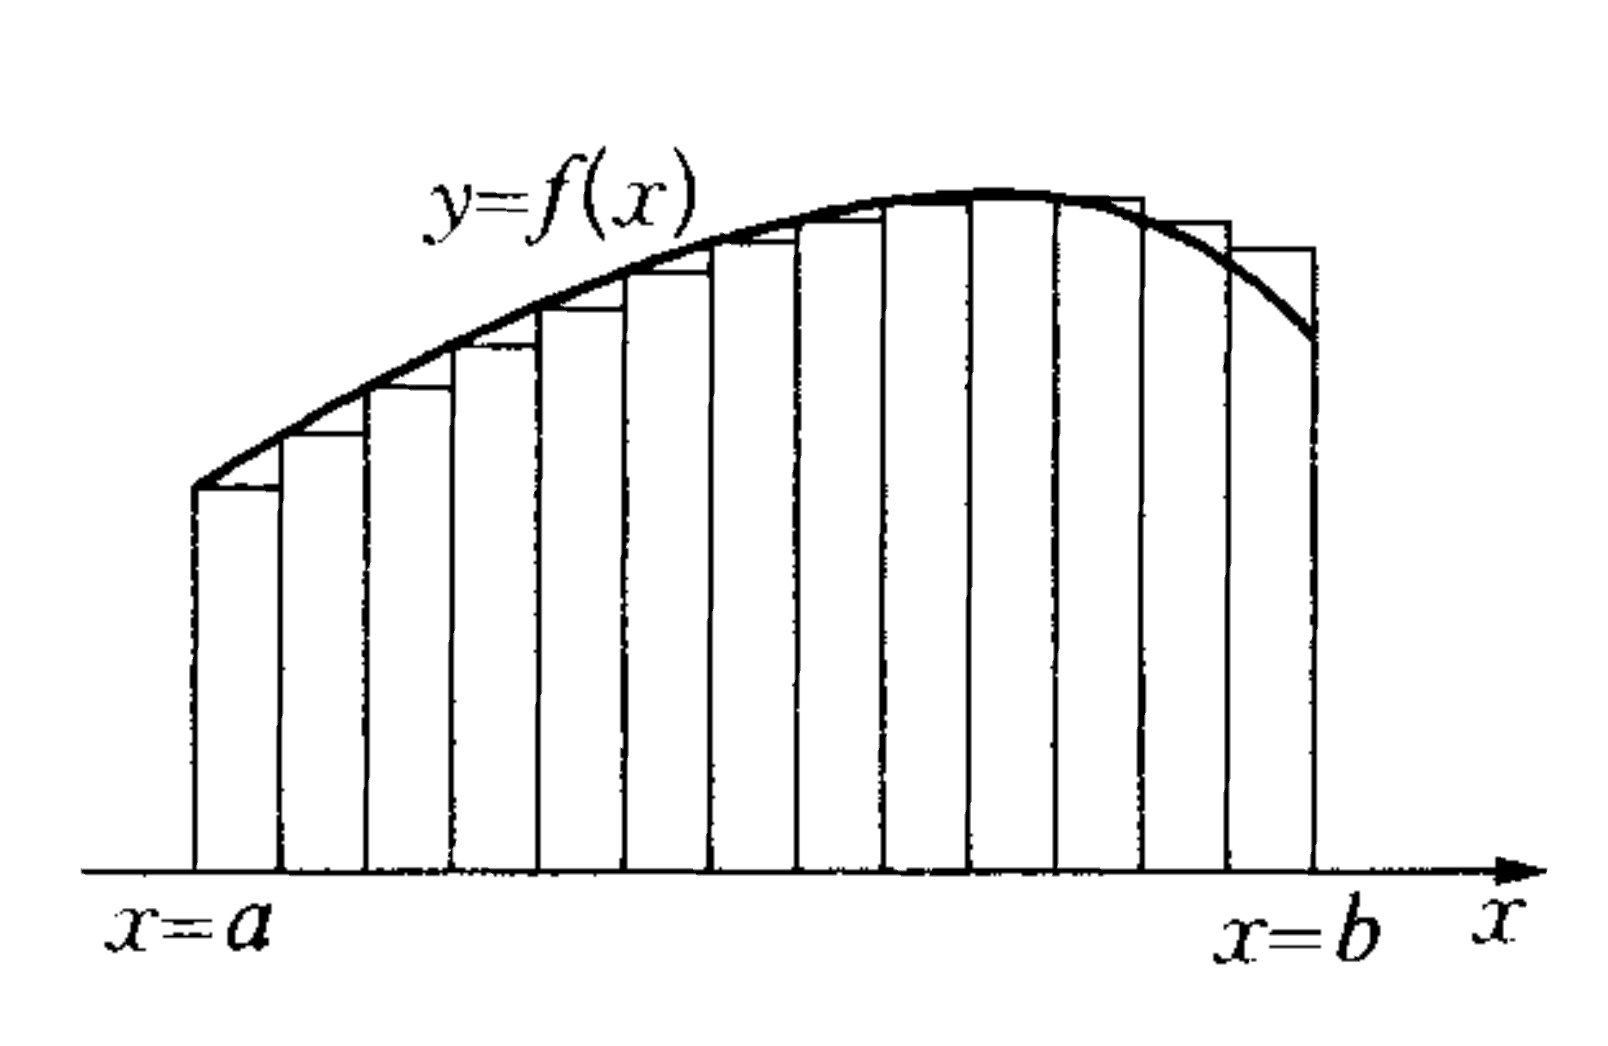
\includegraphics[width=0.8\textwidth]{wine_barrel_function.png}
        \end{figure}
        \begin{figure}
            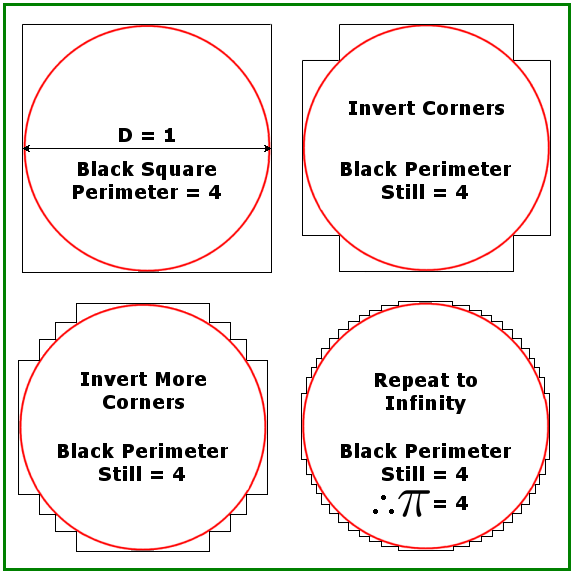
\includegraphics[width=0.7\textwidth]{pi-4.png}
        \end{figure}
    \end{columns}
\end{frame}

\begin{frame}{牛顿: 函数值变化的分析}
    \begin{block}{}
        \begin{enumerate}
            \item   考虑函数 $y=f(x)$;
            \item 	对于自变量 $x_0$, 计算对应的因变量 $f(x_0)$;
            \item 	对于任意增量 $\Delta x$, 可以考察自变量 $x_0+\Delta x$, 并计算对应的因变量 $f(x_0+\Delta x)$;
            \item  	考察自变量增量和因变量增量之间的比值关系:
                  \begin{itemize}
                      \item 自变量的增量为 $\Delta x = x+\Delta x -x$;
                      \item 因变量的增量为 $\Delta y = f(x+\Delta x) -f(x)$;
                      \item 因变量的增量和自变量的增量之比为
                            $$
                                \frac{\Delta y}{\Delta x} = \frac{f(x+\Delta x) -f(x)}{\Delta x};
                            $$
                  \end{itemize}
            \item  考察该比值在 $\Delta x$ 趋于零的情况.
        \end{enumerate}
    \end{block}
    \pause
    {\small	牛顿(Sir Issac Newton, 1643—1727) 在《自然哲学的数学原理》(Philosophiæ Naturalis Principia Mathematica, 1686) 这么解释:
        \pause
        \begin{quote}
            "那些最终比, 随着它们量的消失, 实际上不是最终量的比, 而是无线减小的量的比持续靠近的极限, 他们能比任意给定的差更接近. 但在量被减小以至无穷之前, 既不能超过, 也不能到达此极限." (赵振江译)
        \end{quote}
    }
\end{frame}


\section{动与静的均衡}

\begin{frame}{极限的其他动态描述}

    {\bf 麦克劳林} (Colin Maclaurin, 1698-1746) 在《流数论》 (A treatise on fluxions, 1742): (原文太难找).
    \pause
    {\bf 达朗贝尔} (Jean le Rond d'Alembert, 1717-1783)《百科全书》(Encyclopédie, 1751-1772):
    \begin{quote}
        On l'différentielle ou quantité différentielle, parce qu'on la considere ordinairement comme la différence infiniment petite de deux quantités finies, dont l'une surpasse l'autre infiniment peu.\\
        它被称为微分或微分量,因为它通常被认为是两个有限量之间无限小的差, 其中一个无限小地超过另一个.(DeepL机器翻译)
    \end{quote}
    \pause
    {\bf 柯西} (Augustin-Louis Cauchy, 1789-1857)《微分学教程》(Leçons sur le calcul différentiel, 1829):
    \begin{quote}
        Lorsque les valeurs successivement attribuées à une même variable s'approchent indéfiniment d'une valeur fixe, de manière à finir par en différer aussi peu que l'on voudra, cette dernière est appelée la limite de toutes' les autres.\\
        当连续归属于同一变量的值无限接近一个固定值, 以致最终的差异尽可能小时, 后者被称为所有其他变量的极限.(DeepL机器翻译)
    \end{quote}
\end{frame}

\begin{frame}{魏尔斯特拉斯: 极限的静态描述}
    对照柯西的描述:
    \begin{quote}
        Lorsque les valeurs successivement attribuées à une même variable s'approchent indéfiniment d'une valeur fixe, de manière à finir par en différer aussi peu que l'on voudra, cette dernière est appelée la limite de toutes' les autres.\\
        当属于一个变量的值{\bf \color{red} 无限地趋近}某个固定值时, 以致最终的{\bf\color{blue}差异尽可能小}时, 后者被{\bf \color{green}称为}所有其他变量的极限.(DeepL机器翻译)
    \end{quote}
    \pause
    魏尔斯特拉斯(Karl Weierstrass, 1815-1897) 将这个说明算术化{\small (这里是函数极限的解析描述)}
    \begin{block}{}
        设函数 $f(x)$ 在点 $x=a$ 的某个去心邻域内有定义, 如果存在常数 $L$.\\
        对于任意给定的正实数 $\varepsilon$, 都存在正实数 $\delta$, 使得当 $0 < |x-a| < \delta$ 时, 有 $|f(x) - L| < \varepsilon$ 成立, 则称函数 $f(x)$ 在 $x=a$ 处收敛于 $L$.
    \end{block}
    \pause
    \begin{block}{}
        设函数 $f(x)$ 在点 {\color{red}$x=a$} 的某个去心邻域内有定义, 如果存在{\color{green}常数 $L$}.\\
        {\color{blue}对于任意给定的正实数 $\varepsilon$}, 都存在{\color{red}正实数 $\delta$, 使得当 $0 < |x-a| < \delta$ 时}, {\color{blue}有 $|f(x) - L| < \varepsilon$ 成立}, 则{\color{green} 称函数 $f(x)$ 在 $x=a$ 处收敛于 $L$}.
    \end{block}
\end{frame}

\begin{frame}{魏尔斯特拉斯: 极限的静态描述}
    比较数列极限和函数极限
    \begin{block}{函数极限}
        设函数 $f(x)$ 在点 {\color{red}$x=a$} 的某个去心邻域内有定义, 如果存在{\color{green}常数 $L$}.\\
        {\color{blue}对于任意给定的正实数 $\varepsilon$}, 都存在{\color{red}正实数 $\delta$, 使得当 $0 < |x-a| < \delta$ 时}, {\color{blue}有 $|f(x) - L| < \varepsilon$ 成立}, 则{\color{green} 称函数 $f(x)$ 在 $x=a$ 处收敛于 $L$}.
    \end{block}
    \begin{block}{数列极限}
        考虑数列 $\{x_n\}_{n=1}^\infty$, 如果存在{\color{green}常数 $L$}.\\
        {\color{blue}对于任意给定的正实数 $\varepsilon$}, 都存在{\color{red}正整数 $N$, 使得当正整数 $n\geq N$ 时}, {\color{blue}有 $|x_n - L| < \varepsilon$ 成立}, 则{\color{green} 称数列 $\{x_n\}_{n=1}^\infty$ 收敛于 $L$}.
    \end{block}
\end{frame}

\section{离散与连续的结合}

\begin{frame}{数列极限定义及其扩展}{数列极限的和差公式}
    冯·诺伊曼 (John von Neumann, 1903-1957):
    \begin{quote}
        Young man, in mathematics you don't understand things. You just get used to them.
    \end{quote}
    \pause
    \begin{block}{数列极限$\lim_{n\to\infty}x_n=L$}
        考虑数列 $\{x_n\}_{n=1}^\infty$, 如果存在{\color{green}常数 $L$}.\\
        {\color{blue}对于任意给定的正实数 $\varepsilon$}, 都存在{\color{red}正整数 $N$, 使得当正整数 $n\geq N$ 时}, {\color{blue}有 $|x_n - L| < \varepsilon$ 成立}, 则{\color{green} 称数列 $\{x_n\}_{n=1}^\infty$ 收敛于 $L$}.
    \end{block}
    \pause
    \begin{block}{数列发散$\lim_{n\to\infty}x_n=\infty$}
        考虑数列 $\{x_n\}_{n=1}^\infty$, 如果存在{\color{green}常数 $L$}.\\
        {\color{blue}对于任意给定的正实数 $M$}, 都存在{\color{red}正整数 $N$, 使得当正整数 $n\geq N$ 时}, {\color{blue}有 $x_n > M$ 成立}, 则{\color{green} 称数列 $\displaystyle\lim_{n\to n}x_n=+\infty$.}
    \end{block}
\end{frame}

\begin{frame}{数列极限定义及其扩展}
    \begin{block}{数列极限$\lim_{n\to\infty}x_n=L$}
        考虑数列 $\{x_n\}_{n=1}^\infty$, 如果存在{\color{green}常数 $L$}.\\
        {\color{blue}对于任意给定的正实数 $\varepsilon$}, 都存在{\color{red}正整数 $N$, 使得当正整数 $n\geq N$ 时}, {\color{blue}有 $|x_n - L| < \varepsilon$ 成立}, 则{\color{green} 称数列 $\{x_n\}_{n=1}^\infty$ 收敛于 $L$}.
    \end{block}
    {\small
    \begin{block}{}
        设 $a>1$, 证明: $\lim _{n \rightarrow \infty} \sqrt[n]{a}=1$.
    \end{block}
    \pause
    \begin{exampleblock}{}
        令 $\sqrt[n]{a}=1+y_n, y_n>0(n=1,2,3, \cdots)$, 应用二项式定理,
        $$
            a=\left(1+y_n\right)^n=1+n y_n+\frac{n(n-1)}{2} y_n^2+\cdots+y_n^n>1+n y_n,
        $$

        便得到
        $$
            |\sqrt[n]{a}-1|=\left|y_n\right|<\frac{a-1}{n} .
        $$

        于是, 对于任意给定的 $\varepsilon>0$, 取 $N=\left[\frac{a-1}{\varepsilon}\right]$, 当 $n>N$ 时, 成立
        $|\sqrt[n]{a}-1|<\frac{a-1}{n}<\varepsilon$. 因此 $\lim _{n \rightarrow \infty} \sqrt[n]{a}=1$.
    \end{exampleblock}
    }
\end{frame}

\begin{frame}{数列极限定义及其扩展}
    \begin{block}{}
        求 $\{\sqrt{n+1}-\sqrt{n}\}$ 的极限. (思考题: 求 $\{\sqrt{n^2+1}-\sqrt{n^2-1}\}$ 的极限.)
    \end{block}
    \begin{exampleblock}{}
        由于
        $$
            \sqrt{n+1}-\sqrt{n}=\frac{(\sqrt{n+1}-\sqrt{n})(\sqrt{n+1}+\sqrt{n})}{\sqrt{n+1}+\sqrt{n}}=\frac{1}{\sqrt{n+1}+\sqrt{n}} .
        $$

        取 $x_n=0, y_n=\sqrt{n+1}-\sqrt{n}, z_n=\frac{1}{\sqrt{n}}$, 则有
        $$
            x_n<y_n<z_n,
        $$

        且
        $$
            \lim _{n \rightarrow \infty} x_n=\lim _{n \rightarrow \infty} z_n=0.
        $$

        利用极限的夹逼性, 得到
        $$
            \lim _{n \rightarrow \infty}(\sqrt{n+1}-\sqrt{n})=0 .
        $$
    \end{exampleblock}
\end{frame}

\begin{frame}{数列极限定义及其扩展}{数列极限的和差公式}
    {\small
        \begin{block}{}
            设数列$\{a_n\}$和$\{b_n\}$分别收敛于$a$和$b$, 则它们的乘积数列$\{a_n\pm b_n\}$也收敛, 并且有以下性质:
            \begin{itemize}
                \item $\lim\limits_{n \to \infty}(a_n \pm b_n) = a \pm b$.
            \end{itemize}
        \end{block}
        \pause
        \begin{exampleblock}{}
            对于和差数列$\{a_n \pm b_n\}$, 我们需要证明它们分别收敛于$a + b$和$a - b$.

            首先, 根据数列的收敛性定义, 对于任意给定的正数$\varepsilon_1$, 存在正整数$N_1(\varepsilon_1)$, 当$n > N_1(\varepsilon_1)$时, 有$|a_n - a| < \varepsilon_1$; 同样地, 对于任意给定的正数$\varepsilon_2$, 存在正整数$N_2(\varepsilon_2)$, 当$n > N_2(\varepsilon_2)$时, 有$|b_n - b| < \varepsilon_2$.\\
            \vspace{0.2cm}
            对于 $\varepsilon$. 我们选择正整数$N = \max(N_1(\frac{\varepsilon}{2}), N_2(\frac{\varepsilon}{2}))$, 则当$n > N$时, 有:
            \begin{align*}
                |(a_n + b_n) - (a + b)| & = |(a_n - a) + (b_n - b)|                                              \\
                                        & \leq |a_n - a| + |b_n - b|                                             \\
                                        & < \frac{\varepsilon}{2} + \frac{\varepsilon}{2} \leqslant \varepsilon.
            \end{align*}
            同理, 我们可以证明$|(a_n - b_n) - (a - b)| < \varepsilon$.

            因此, 根据数列的收敛性定义, $\{a_n \pm b_n\}$分别收敛于$a + b$和$a - b$.
        \end{exampleblock}
    }
\end{frame}

\begin{frame}{数列极限定义及其扩展}{数列极限的乘积公式}
    \begin{block}{数列乘积极限}
        考虑数列 $\{x_n\}_{n=1}^\infty$, 如果存在{\color{green}常数 $L$}.\\
        {\color{blue}对于任意给定的正实数 $\varepsilon$}, 都存在{\color{red}正整数 $N$, 使得当正整数 $n\geq N$ 时}, {\color{blue}有 $|x_n - L| < \varepsilon$ 成立}, 则{\color{green} 称数列 $\{x_n\}_{n=1}^\infty$ 收敛于 $L$}.
    \end{block}
    \begin{block}{}
        设数列$\{a_n\}$和$\{b_n\}$分别收敛于$a$和$b$, 则它们的乘积数列$\{a_nb_n\}$也收敛, 并且有以下性质:
        \begin{itemize}
            \item $\lim\limits_{n \to \infty}(a_n  b_n) = a b$.
        \end{itemize}
    \end{block}
\end{frame}
\begin{frame}{数列极限定义及其扩展}{数列极限的乘积公式}
    \begin{block}{}
        对于乘积数列$\{a_n b_n\}$, 我们需要证明它们收敛于$a b$.

        首先, 根据数列的收敛性定义, 对于任意给定的正数$\varepsilon_1$, 存在正整数$N_1(\varepsilon_1)$, 当$n > N_1(\varepsilon_1)$时, 有$|a_n - a| < \varepsilon_1$; 同样地, 对于任意给定的正数$\varepsilon_2$, 存在正整数$N_2(\varepsilon_2)$, 当$n > N_2(\varepsilon_2)$时, 有$|b_n - b| < \varepsilon_2$.\\
        \vspace{0.2cm}
        我们首先考虑$a,b\neq0$的情况. 对于 $\varepsilon$, 我们选择正整数$N = \max(N_1(\frac{\varepsilon}{2|b|}), N_2(\frac{\varepsilon}{4|a|}))$, 则当$n > N$时, 利用极限的保号性,有:
        \begin{align*}
            |(a_n b_n) - (a  b)| & = |a_n(b_n - b)+(a_n - a)b|                                    \\
                                 & \leq |a_n||(b_n - b)|+|(a_n - a)||b|                           \\
                                 & < 2|a||(b_n - b)|+|(a_n - a)||b|                               \\
                                 & < 2|a|\frac{\varepsilon}{4|a|} + |b|\frac{\varepsilon}{2|b|}   \\
                                 & < \frac{\varepsilon}{2} + \frac{\varepsilon}{2} = \varepsilon.
        \end{align*}
    \end{block}
\end{frame}


\begin{frame}{数列极限定义及其扩展}{数列极限的商公式}
    \begin{block}{}
        考虑$a,b$ 其中一个为零的情况, 不放设 $b=0$ 对于 $\varepsilon$, 我们选择正整数$N = \max(N_1(|a|), N_2(\frac{\varepsilon}{2|a|}))$, 则当$n > N$时, 利用极限的保号性,有:
        \begin{align*}
            |(a_n b_n)| & \leq |a_n||b_n|\leq 2|a|\cdot\frac{\varepsilon}{2|a|}.
        \end{align*}
        \vspace{0.5cm}
        考虑$a,b$ 全为零的情况.  对于 $\varepsilon$, 我们选择正整数$N = \max(N_1(1),N_2(\varepsilon))$, 则当$n > N$时, 利用极限的保号性,有:
        \begin{align*}
            |(a_n b_n)| & \leq |a_n||b_n|\leq 1\cdot\varepsilon\leq \varepsilon.
        \end{align*}
        因此, 根据数列的收敛性定义, $\{a_n  b_n\}$收敛于$a  b$.\\\qed
    \end{block}
\end{frame}


\begin{frame}{数列极限定义及其扩展}{数列极限的乘积公式}
    \begin{block}{数列极限}
        考虑数列 $\{x_n\}_{n=1}^\infty$, 如果存在{\color{green}常数 $L$}.\\
        {\color{blue}对于任意给定的正实数 $\varepsilon$}, 都存在{\color{red}正整数 $N$, 使得当正整数 $n\geq N$ 时}, {\color{blue}有 $|x_n - L| < \varepsilon$ 成立}, 则{\color{green} 称数列 $\{x_n\}_{n=1}^\infty$ 收敛于 $L$}.
    \end{block}
    \begin{block}{}
        设数列$\{a_n\}$和$\{b_n\}$分别收敛于$a$和$b$, 而且 $b\neq0$, 则它们的商数列$\{\frac{a_n}{b_n}\}$也收敛, 并且有以下性质:
        \begin{itemize}
            \item $\lim\limits_{n \to \infty}\left(\displaystyle\frac{a_n}{b_n}\right) = \displaystyle\frac{a}{b}$.
        \end{itemize}
    \end{block}
\end{frame}

\begin{frame}{数列极限定义及其扩展}{数列极限的商公式}
    \begin{block}{}
        由于极限的乘积公式, 我们实际上只需要讨论
        \[
            \lim_{n\to\infty}\frac{1}{b_n}=\frac{1}{b}.
        \]
        由 $b_n$ 收敛的定义.  对于任意给定的正数$\varepsilon_1$, 存在正整数$N_1(\varepsilon_1)$, 当$n > N_1(\varepsilon_1)$时, 有$|b_n - b| < \varepsilon_1$. 对于 $\varepsilon$. 我们选择正整数$N = \max(N_1(\frac{|b|^2\varepsilon}{2}), N_1(\frac{|b|}{2}))$, 则当$n > N$时, 利用极限的保号性,有:
        \begin{align*}
            \left|\frac{1}{b_n}-\frac{1}{b}\right| & = \frac{|b_n-b|}{|b||b_n|}<\frac{\frac{|b|^2\varepsilon}{2}}{\frac{|b|^2}{2}}\leq\varepsilon.
        \end{align*}
        因此, 根据数列的收敛性定义, $\{\frac{a_n}{b_n}\}$收敛于$\frac{a}{b}$.\\\qed
    \end{block}
\end{frame}

\begin{frame}{数列极限定义及其扩展}{Bolzano-Weierstrass定理: 有界数列都有收敛子列}
    \begin{exampleblock}{}
        设数列 $\left\{x_n\right\}$ 有界, 于是存在实数 $a_1, b_1$, 成立$a_1 \leqslant x_n\leqslant b_1$,接下来
        \begin{enumerate}
            \item 将闭区间 $\left[a_1, b_1\right]$ 等分为两个小区间 $\left[a_1, \frac{a_1+b_1}{2}\right]$ 与 $\left[\frac{a_1+b_1}{2}, b_1\right]$, 则其中至少有一个含有数列 $\left\{x_n\right\}$ 中的无穷多项, 把它记为 $\left[a_2, b_2\right]$.
            \item 再将闭区间 $\left[a_2, b_2\right]$ 等分为两个小区间 $\left[a_2, \frac{a_2+b_2}{2}\right]$ 与 $\left[\frac{a_2+b_2}{2}, b_2\right]$, 同样其中至少有一个含有数列 $\left\{x_n\right\}$ 中的无穷多项, 把它记为 $\left[a_3, b_3\right]$.
            \item  这样的步骤可以一直做下去, 于是得到一个闭区间套 $\left\{\left[a_k, b_k\right]\right\}$, 其中每一个闭区间 $\left[a_k, b_k\right]$ 中都含有数列 $\left\{x_n\right\}$ 中的无穷多项.
            \item 这个闭区间套存在极限 $\displaystyle\xi=\lim_{n\to\infty}a_n=\lim_{n\to\infty}b_n$.
            \item 取子列 $\{x_{n_k}\}$ 如下:
                  \begin{enumerate}
                      \item $n_1=1$;
                      \item 对任意 $k\ge2$, 取$n_k\ge n_{k-1}$ 且 $x_{n_k}\in [a_{k},b_{k}]$
                  \end{enumerate}
            \item 由于对任意 $k\ge2$, $[a_{k},b_{k}]$ 内均有无穷多项, 这个过程可以经历任意有限次.
            \item 由三明治法则, 该子列$\{x_{n_k}\}$ 满足 $a_k\leq x_{n_k}\leq b_k$, 其极限为$\xi$.\qed
        \end{enumerate}
    \end{exampleblock}
\end{frame}

\begin{frame}{函数极限相关}
    \begin{block}{函数极限$\lim_{x\to a}f(x)=L$}
        设函数 $f(x)$ 在点 {\color{red}$x=a$} 的某个去心邻域内有定义, 如果存在{\color{green}常数 $L$}.\\
        {\color{blue}对于任意给定的正实数 $\varepsilon$}, 都存在{\color{red}正实数 $\delta$, 使得当 $0 < |x-a| < \delta$ 时}, {\color{blue}有 $|f(x) - L| < \varepsilon$ 成立}, 则{\color{green} 称函数 $f(x)$ 在 $x=a$ 处收敛于 $L$}.
    \end{block}
    \pause
    \begin{block}{函数极限$\lim_{x\to a}f(x)=-\infty$}
        设函数 $f(x)$ 在点 {\color{red}$x=a$} 的某个去心邻域内有定义, {\color{blue}对于任意给定的正实数 $M$}, 都存在{\color{red}正实数 $\delta$, 使得当 $0 < |x-a| < \delta$ 时}, {\color{blue}有 $f(x) < -M$ 成立}, 则$\displaystyle\lim_{x\to a}f(x)=-\infty$.
    \end{block}
    \pause
    \begin{block}{函数极限$\lim_{x\to +\infty}f(x)=L$}
        设函数 $f(x)$ 在区间 $(a,\infty)$ 上有定义 (其中$a$为常数), 如果存在{\color{green}常数 $L$}.\\
        {\color{blue}对于任意给定的正实数 $\varepsilon$}, 都存在{\color{red}正实数 $X$, 使得当 $x> X$ 时}, {\color{blue}有 $|f(x) - L| < \varepsilon$ 成立}, 则{\color{green} 称函数 $f(x)$ 在正无穷远处收敛于 $L$}.
    \end{block}
    类似地, 可以写出一系列收敛/趋于正无穷/趋于负无穷/趋于无穷的定义.
\end{frame}

\begin{frame}
    \frametitle{函数极限相关}
    \begin{block}{}
        证明: $\lim _{x \rightarrow+\infty} e^{-x}=0$.
    \end{block}
    \pause
    \begin{proof}
        对于任意给定的$\varepsilon>0$, 存在正数$M$, 使得当$x > M$时, 有
        $$
            e^{-x} < \varepsilon.
        $$
        我们可以取 $M=\log (\varepsilon^{-1})$ 有$x > M$,
        $$
            x>\log(\varepsilon^{-1}),\,\,\log\varepsilon>-x,\,\,\text{即}\,\,\varepsilon>-x.
        $$
    \end{proof}
\end{frame}

\begin{frame}{函数极限相关}
    \begin{block}{}
        证明: $\lim _{x \rightarrow 1^-} \frac{x^2}{x-1}=-\infty$.
    \end{block}
    \pause
    \begin{proof}
        对于任意给定的 $M>0$, 要找 $\delta>0$, 使当 $-\delta<x-1<0$ 时成立
        $$
            \frac{x^2}{x-1}<-G
        $$

        为了适度放大不等式的左边, 先加上条件 $-\frac{1}{2}<x-1<0$, 于是 $x^2>\frac{1}{4}$, 从而 $\frac{x^2}{x-1}<$ $\frac{1}{4(x-1)}$. 令 $\delta=\min \left\{\frac{1}{2}, \frac{1}{4 M}\right\}$, 则当 $-\delta<x-1<0$ 时
        $$
            \frac{x^2}{x-1}<\frac{1}{4(x-1)}<-\frac{1}{4 \delta} \leqslant-M .
        $$

        由此证得 $\lim _{x \rightarrow 1^-} \frac{x^2}{x-1}=-\infty$.
    \end{proof}
\end{frame}

\begin{frame}{函数极限相关}
    \begin{theorem}[Heine]
        $\lim _{x \rightarrow x_0} f(x)=A$ 的充分必要条件是: 对于任意满足条件 $\lim _{n \rightarrow \infty} x_n=x_0$, 且 $x_n \neq x_0(n=1,2,3, \cdots)$ 的数列 $\left\{x_n\right\}$, 相应的函数值数列 $\left\{f\left(x_n\right)\right\}$ 成立 $\lim _{n \rightarrow \infty} f\left(x_n\right)=A$.
    \end{theorem}
    \pause
    \begin{block}{}
        必要性: 由 $\lim _{x \rightarrow x_0} f(x)=A$ 可知,
        $$
            \forall \varepsilon>0, \exists \delta>0, \forall x\left(0<\left|x-x_0\right|<\delta\right):|f(x)-A|<\varepsilon .
        $$

        因为 $\lim _{n \rightarrow \infty} x_n=x_0$, 且 $x_n \neq x_0(n=1,2,3, \cdots)$, 对于上述 $\delta>0, \exists N, \forall n>N$ :
        $$
            0<\left|x_n-x_0\right|<\delta \text {. }
        $$

        于是当 $n>N$ 时,成立
        $$
            \left|f\left(x_n\right)-A\right|<\varepsilon,
        $$

        即 $\lim _{n \rightarrow \infty} f\left(x_n\right)=A$.
    \end{block}
\end{frame}

\begin{frame}{函数极限相关}
    \begin{block}{}
        充分性: 用反证法.
        按函数极限定义, 命题 “ $f(x)$ 在 $x_0$ 点以 $A$ 为极限” 可以表述为
        $$
            \forall \varepsilon>0, \exists \delta>0, \forall x\left(0<\left|x-x_0\right|<\delta\right):|f(x)-A|<\varepsilon .
        $$

        于是它的否定命题 “ $f(x)$ 在 $x_0$ 点不以 $A$ 为极限” 可以对偶地表述为
        $$
            \exists \varepsilon_0>0, \forall \delta>0, \exists x\left(0<\left|x-x_0\right|<\delta\right):|f(x)-A| \geqslant \varepsilon_0 .
        $$
        现在取一列 $\left\{\delta_n\right\}, \delta_n=\frac{1}{n}(n=1,2,3, \cdots)$.\\
        对 $\delta_1=1$, 存在 $x_1\left(0<\left|x_1-x_0\right|<\delta_1\right)$, 使 $\left|f\left(x_1\right)-A\right| \geqslant \varepsilon_0$;\\
        对 $\delta_2=\frac{1}{2}$, 存在 $x_2\left(0<\left|x_2-x_0\right|<\delta_2\right)$, 使 $\left|f\left(x_2\right)-A\right| \geqslant \varepsilon_0$;\\
        \vspace{0.1cm}
        $\cdots\cdots$\\
        \vspace{0.1cm}
        一般地, 对 $\delta_k=\frac{1}{k}$, 存在 $x_k\left(0<\left|x_k-x_0\right|<\delta_k\right)$, 使 $\left|f\left(x_k\right)-A\right| \geqslant \varepsilon_0$.\\
        
        \vspace{0.2cm}
        于是得到数列 $\left\{x_n\right\}$, 满足 $x_n \neq x_0, \lim _{n \rightarrow \infty} x_n=x_0$, 但相应的函数值数列 $\left\{f\left(x_n\right)\right\}$ 不可能以 $A$ 为极限.\qed
    \end{block}
\end{frame}

% Thank you page
\beamertemplateshadingbackground{structure.fg!90}{structure.fg}
\begin{frame}[plain]
    \vfill
    \centering
    {
    \centering \Huge \color{white} Thank you for your attention!\\[10pt]Questions?\\ [10pt] Homework:\\{$\{\sqrt{n^2+1}-\sqrt{n^2-1}\}$ 的极限.}\\ 证明:\\函数和差的极限公式, \\函数商的极限公式.
    }
    \vfill
\end{frame}


\end{document}


